\documentclass{beamer}

\usepackage{emoji}

\usetheme{PSY9511}

\title{Russell's Paradox}
\author{Esten H. Leonardsen}
\date{10.02.25}


\begin{document}
	\begin{frame}
	 	\maketitle
	\end{frame}

    \begin{frame}{Background}
        \begin{tikzpicture}
            \node[] at (-5.25, -3.5) {};
            \node[] at (5.25, 3.5) {};

            \visible<1-2>{
                \node[inner sep=0pt, draw=black, rotate=90] at (-2.675, 0) {
                    \includegraphics[width=5cm]{data/tattoo.jpg}
                };
            }
            \visible<2>{
                \node[] at (2.675, 0) {
                    $\{S | S \notin S\}$
                };
            }
            \visible<3>{
                \node[inner sep=0pt, draw=black, label=below:\tiny{Source: A guy I met at a party once}] at (0, 0) {
                    
\includegraphics[width=9cm]{data/westworld.jpg}
                };
            }
        \end{tikzpicture}
    \end{frame}

    \begin{frame}{Historical underpinnings}
        \begin{tikzpicture}
            \node[draw=black] at (-5.25, -3.5) {};
            \node[draw=black] at (5.25, 3.5) {};

            \visible<1>{
                \node[inner sep=0pt, draw=black] at (0, 0) {
                    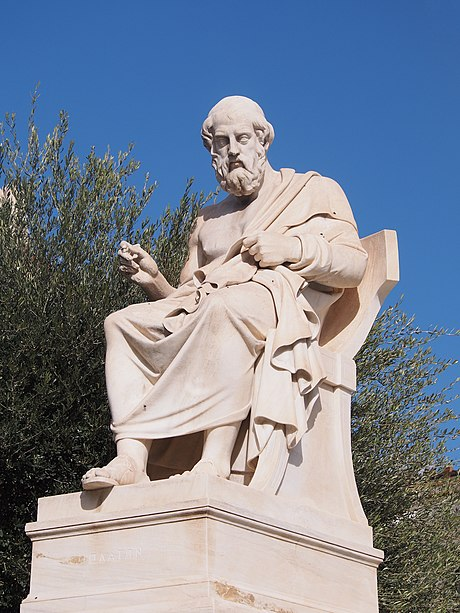
\includegraphics[width=4.5cm]{data/plato.JPG}
                };
            }
            \visible<2>{
                \node[inner sep=0pt, draw=black] at (0, 0) {
                    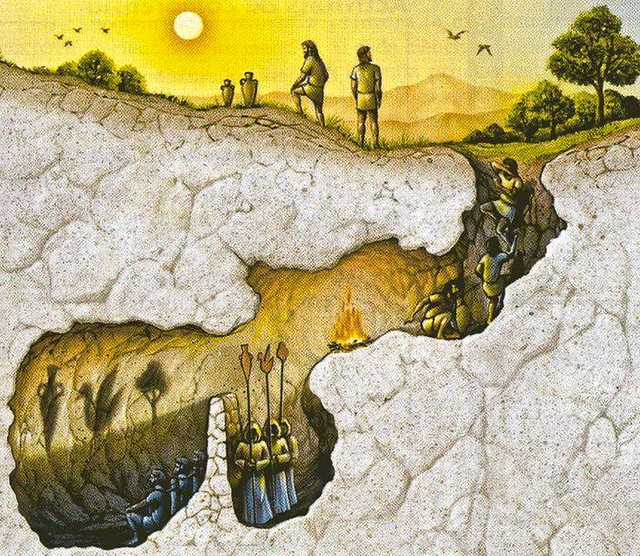
\includegraphics[width=7.5cm]{data/cave.jpg}
                };
            }
            \visible<3>{
                \node[inner sep=0pt, draw=black] at (0, 0) {
                    
\includegraphics[width=6cm]{data/kant.jpeg}
                };
            }
            \visible<4-5>{
                \node[inner sep=0pt, draw=black] at (-2.675, 0) {
                    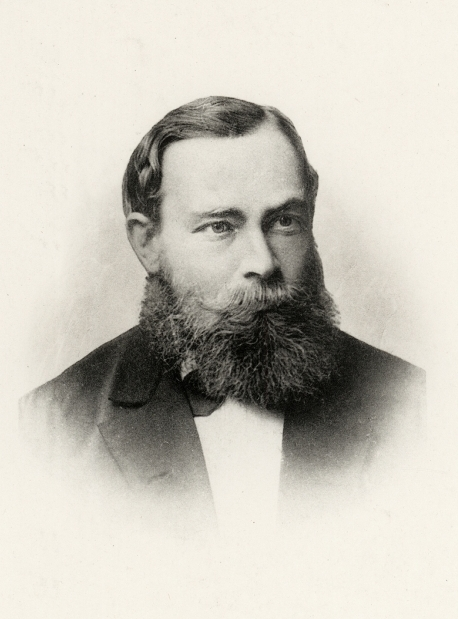
\includegraphics[height=5cm]{data/frege.jpg}
                };
            }
            \visible<5>{
                \node[inner sep=0pt, draw=black] at (2.675, 0) {
                    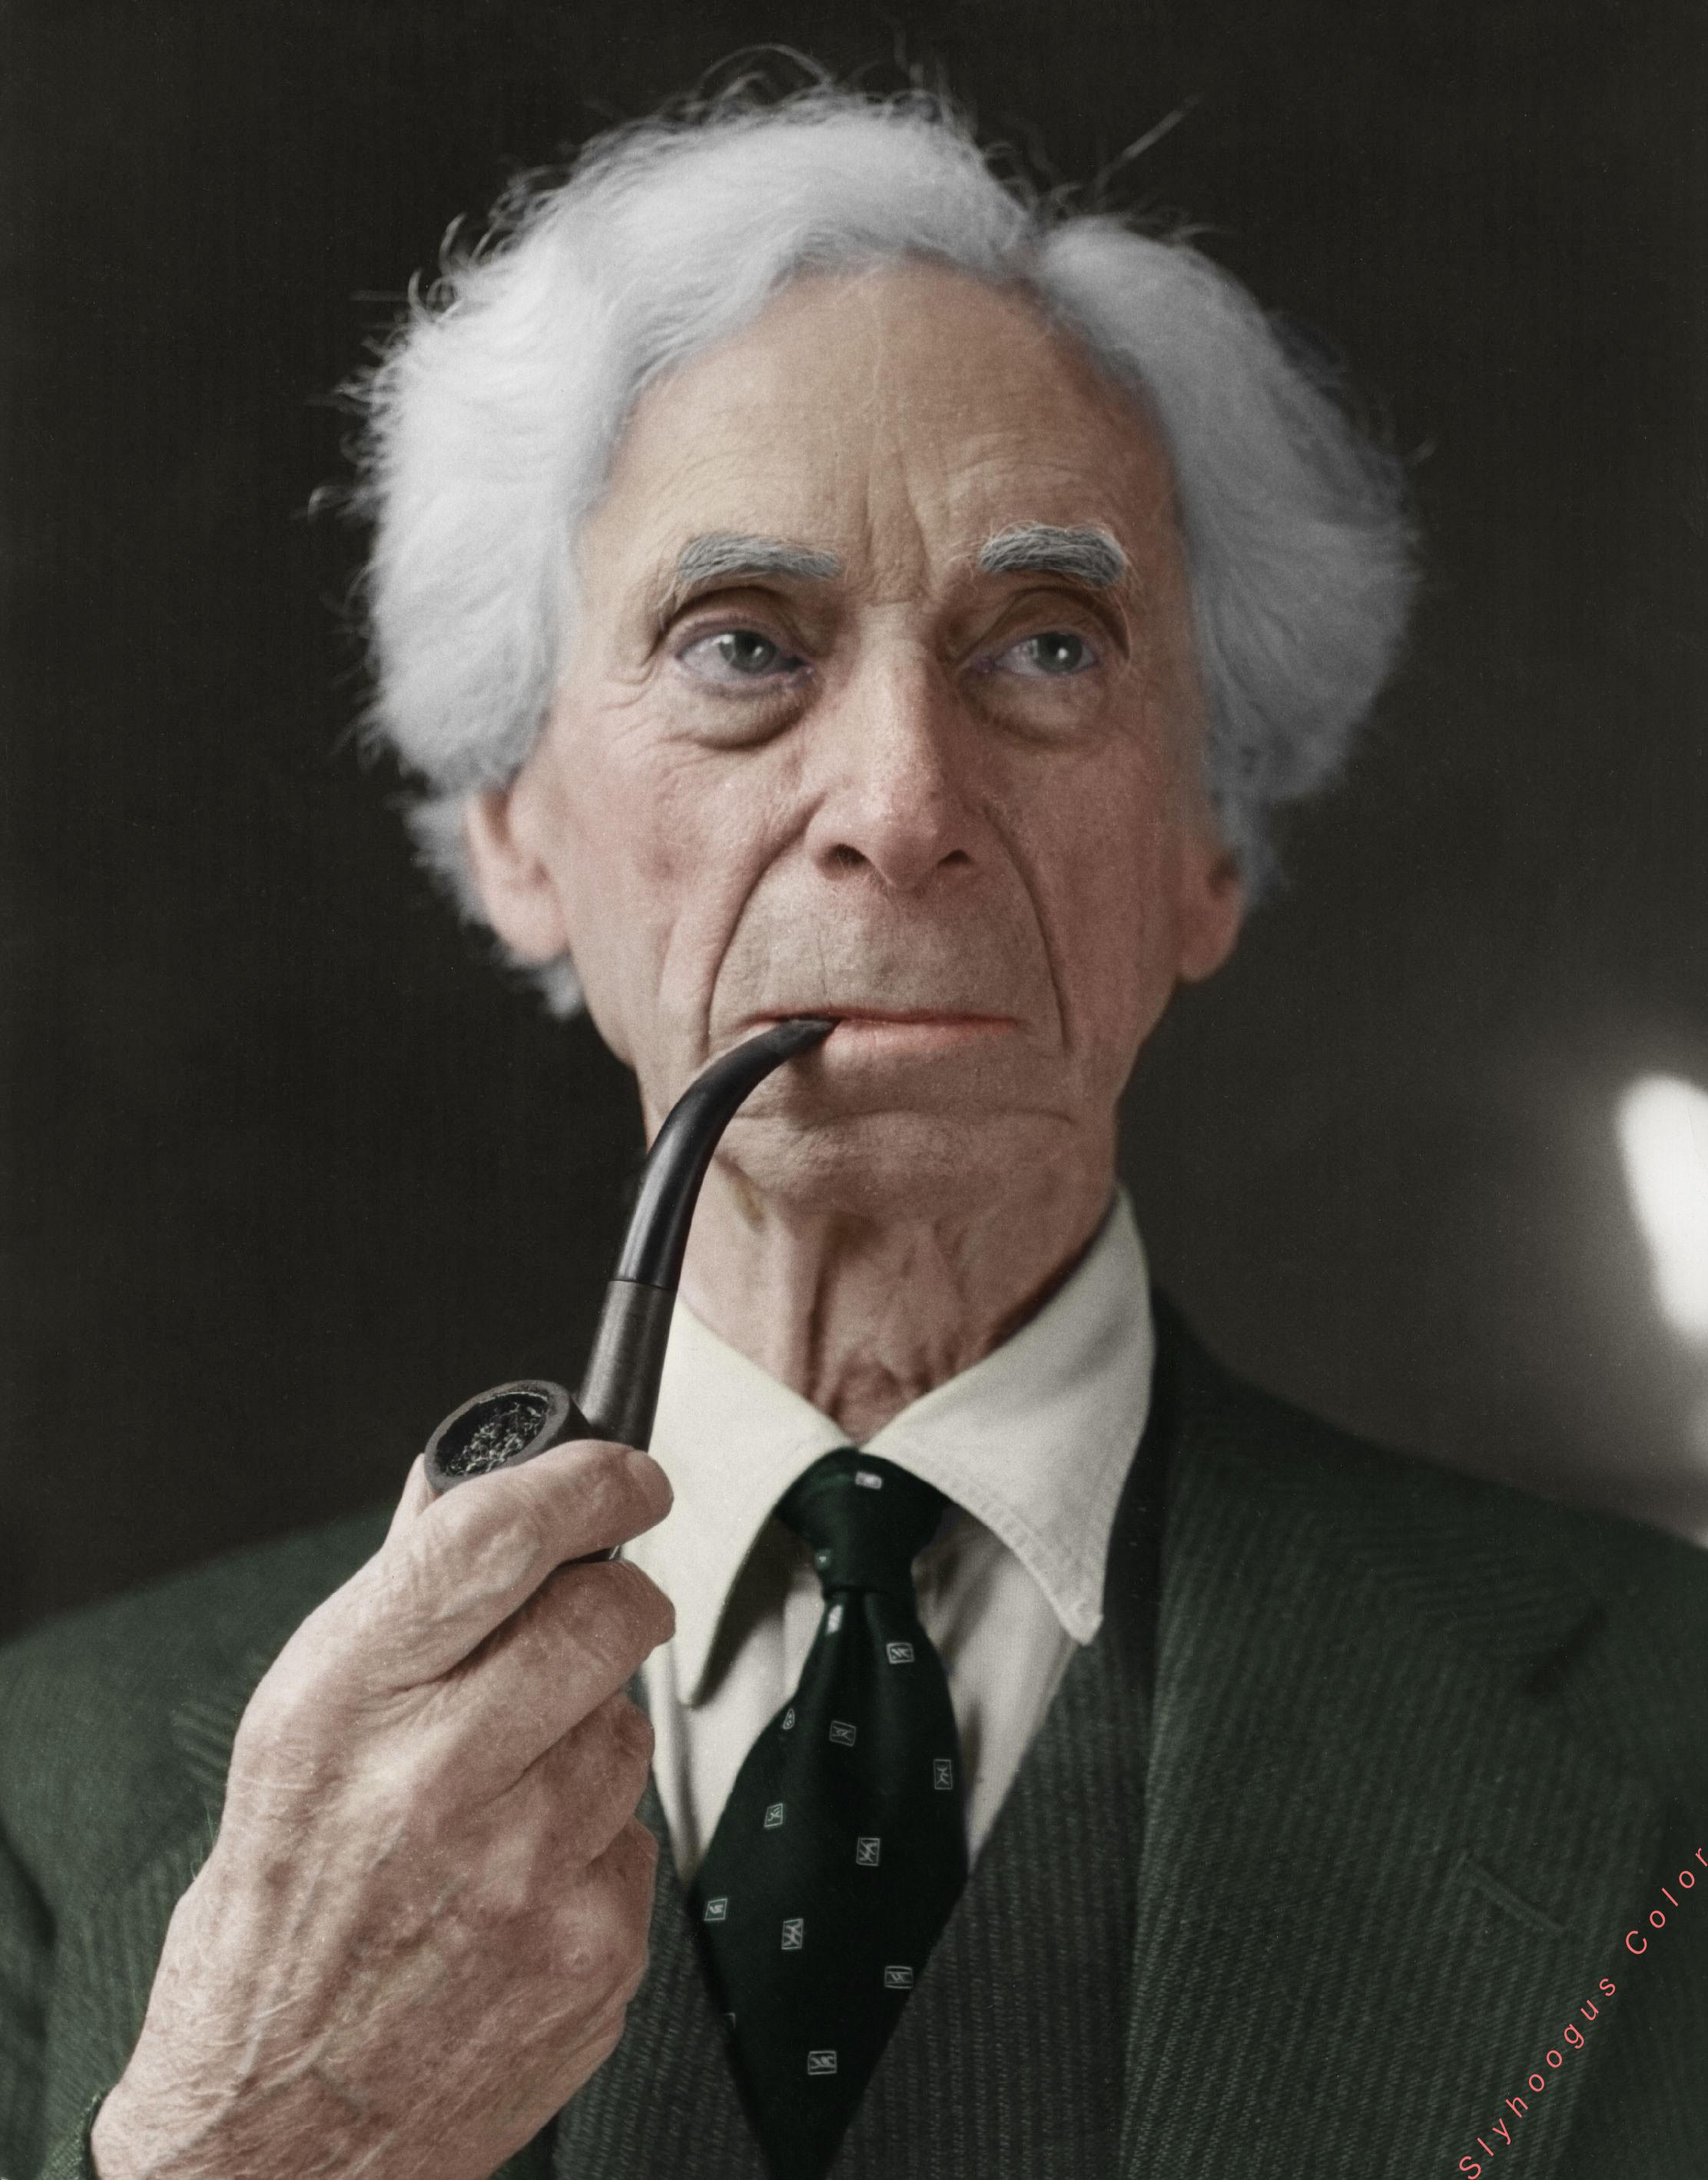
\includegraphics[height=5cm]{data/russell.jpg}
                };
            }
        \end{tikzpicture}
    \end{frame}

    \begin{frame}{The project}
        \begin{tikzpicture}
            \node[] at (-5.25, -3.5) {};
            \node[] at (5.25, 3.5) {};

            \visible<1-2>{
                \node[align=center] (functions) at (-2.675, -1) {
                    $x+y=z$\\$x-y=z$\\\ldots
                };
                \node[] (numbers) at (-2.675, 1) {
                    $0, 1, 2, 3, 4, \ldots$
                };
            }
            \visible<2>{
                \node[] at (0, 1) {
                    $\implies$
                };
                \node[] at (0, -1) {
                    $\implies$
                };
                \node[] at (2.675, 1) {
                    \large{\emoji{thinking-face}}
                };
                \node[] at (2.675, -1) {
                    \large{\emoji{check-mark-button}}
                };
            }
        \end{tikzpicture}
    \end{frame}

    \begin{frame}{Set theory}
        \begin{tikzpicture}
            \node[] at (-5.25, -3.5) {};
            \node[] at (5.25, 3.5) {};

            \visible<1>{
                \node[inner sep=0pt, draw=black] at (0, 0) {
                    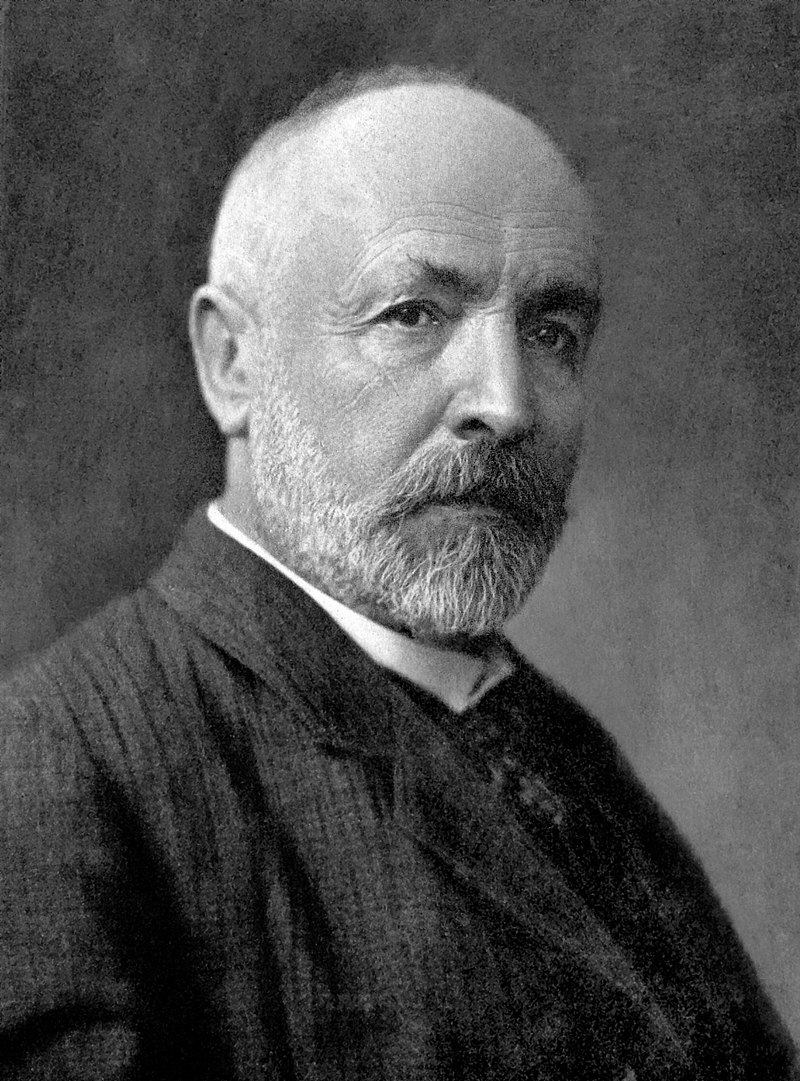
\includegraphics[width=5cm]{data/cantor.jpg}
                };
            }
            \visible<2>{
                \node[] at (0, 1.5) {
                    \{\emoji{nerd-face}, \emoji{woman}, \emoji{girl}, \emoji{dog-face}\}
                };
                \node[] at (0, 0.5) {
                    \{\emoji{nerd-face}, \emoji{smiling-face-with-sunglasses}, \emoji{face-with-monocle}, \emoji{woman-scientist},
                    \emoji{woman-technologist}, \emoji{woman-teacher}\}
                };
                \node[align=center] at (0, -0.5) {
                    \{monday, tuesday, wednesday, thursday,\\friday, saturday, sunday\}
                };
                \node[] at (0, -1.5) {
                    \{\emoji{laptop}, \emoji{mobile-phone}\}
                };
            }
            \visible<3>{
                \node[] at (0, 1) {
                    $\{1, 3, 5\}$
                };
                \node[] at (0, 0) {
                    $\{1, 10, 100\}$
                };
                \node[align=center] at (0, -1) {
                    $\{\}$
                };
            }
            \visible<4-6>{
                \node[] at (0, 1.5) {
                    $\{0, 1, 2, \ldots, 9999, 10000\}$
                };
            }
            \visible<5-6>{
                \node[] at (0, 0.5) {
                    $\{x\ |\ x \leq 10000\}$
                };
            }
            \visible<6>{
                \node[] at (0, -0.5) {
                    $\{1, 3, 5, \ldots\}$
                };
                \node[] at (0, -1.5) {
                    $\{x\ |\ x\ \%\ 2 = 1\}$
                };
            }
        \end{tikzpicture}
    \end{frame}

\end{document}
